\documentclass[20pt]{beamer}


\usetheme{hm}

\setbeamertemplate{section in toc}[sections numbered]
\setbeamertemplate{subsection in toc}[subsections numbered]

% Subsecciones (indentadas)
\setbeamertemplate{subsection in toc}{
  \hspace*{3.0em}% <<< INDENTACIÓN
  \llap{\inserttocsectionnumber.\inserttocsubsectionnumber\ }%
  \inserttocsubsection\par
}

\usepackage{minted}
\usepackage{tikz}
\usepackage{caption}
\usepackage{subfigure}
\usepackage{tcolorbox}

% Kein Dekor auf Titelfolie
%\usetheme[nodecotitle]{hm}

% Kein Dekor auf anderen Folien
%\usetheme[nodeco]{hm}

% Logo im Titel und nicht unten (für wide&nodeco interessant)
%\usetheme[logotop]{hm}

% Keine Foliennummer
%\usetheme[noframenum]{hm}

% Creative Commons CC-BY Lizenz
%\usetheme[ccby]{hm}

\author{Daniel Arevalos}
\institute{Munich University of Applied Sciences HM}
\title{ShapeIC: Design-Space Exploration}
%\title{Vorlesung I mit einem langen Titel über zwei Zeilen}
\subtitle{Hierarchical LUT-based design-space exploration for analog IC sizing}
%\subtitle{Kapitel 1 -- Eine Einführung die über zwei Zeilen geht und trotzdem gut passt}


\begin{document}

\begin{frame}[plain]
\titlepage
\end{frame}

%\setlength{\parskip}{0mm}
%\begin{frame}
%\frametitle{Table of Contents}
%\vspace{3cm}
%\tableofcontents
%\vspace{2cm}
%\end{frame}

\section{Analog Sizing: Optimize or Explore ?}

\begin{frame}{Automatic Analog Sizing}
\begin{columns}
    \begin{column}{0.45\textwidth}
      \begin{itemize}
        \item<2-> Optimization-driven 
      \end{itemize}
      \uncover<2->{
          \center
          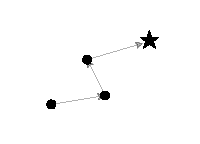
\includegraphics[width=0.6\textwidth]{img/optimization-driven.pdf}
      } 
      \begin{itemize}
        \item<2->[\checkmark] Strategic evaluation of candidates
        \item<2->[\checkmark] Many algorithms available
      \end{itemize}
      \begin{itemize}
        \item<3->[$\times$] Partial View of the design space
        \item<3->[$\times$] May converge to local optima
      \end{itemize}
    \end{column}
    \begin{column}{0.45\textwidth}
      \begin{itemize}
        \item<4-> Design-space exploration
      \end{itemize}
      \uncover<4->{
          \center
          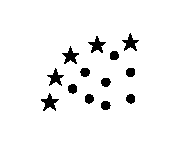
\includegraphics[width=0.6\textwidth]{img/design-space-exploration.pdf}
      }
      \begin{itemize}
        \item<4->[\checkmark] Design insight
        \item<4->[\checkmark] Alternative solutions
      \end{itemize}
      \begin{itemize}
        \item<5->[$\times$] Expensive to build
        \item<5->[$\times$] Scales poorly without abstraction
      \end{itemize}
    \end{column}
\end{columns}

\end{frame}

\begin{frame}
  \frametitle{Let's explore a 2 Stage Amplifier}
\begin{columns}
    \begin{column}{0.45\textwidth}
      \center
      \only<2>{
        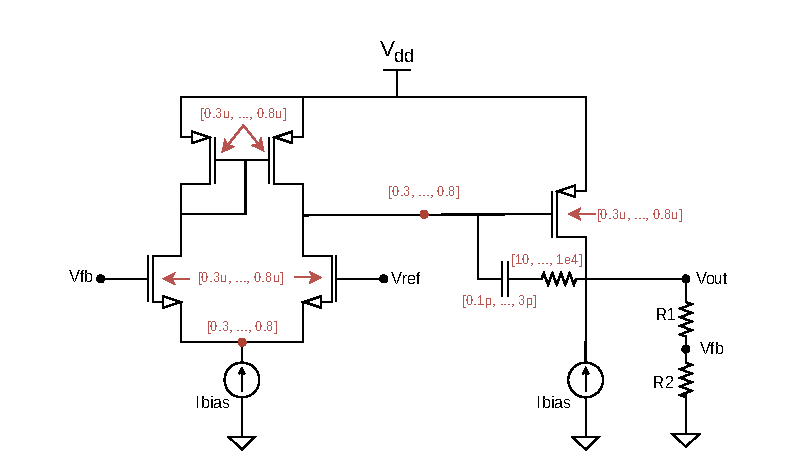
\includegraphics[width=1.1\textwidth]{img/ota_2stage-params.pdf} 
      }
      \only<1>{
        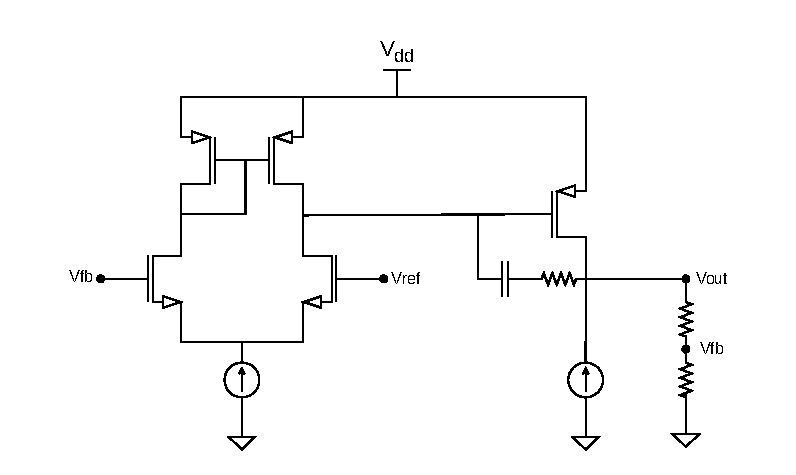
\includegraphics[width=1.1\textwidth]{img/ota_2stage-pre.pdf} 
      }
      \only<3>{
        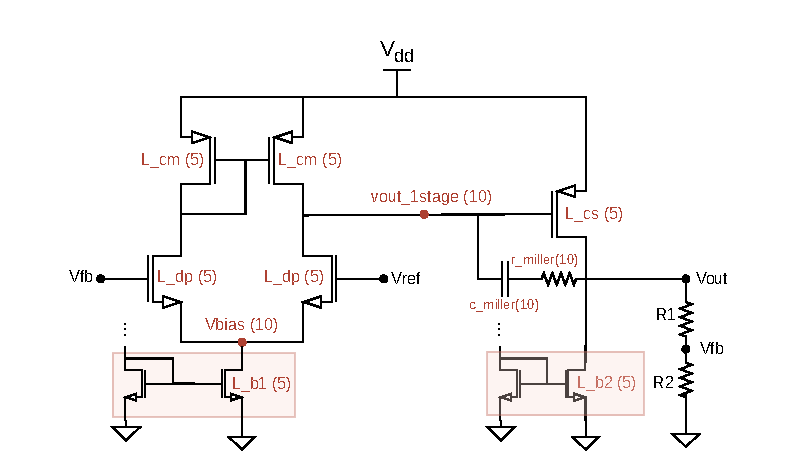
\includegraphics[width=1.1\textwidth]{img/ota_2stage-params-2.pdf} 
      }
    \end{column}
    \begin{column}{0.45\textwidth}
      \begin{itemize}
        \item<1-> Simple 5 transistor topology
        \item<2-> 1250000 design candidates
          \begin{itemize}
            \item Simulation: $\approx2h$
            \item Equation evaluations: $\approx2s$ (derived by hand)
          \end{itemize}
        \item<3-> 31250000 design candidates
          \begin{itemize}
            \item Simulation: $\approx1 month$ 
            \item Equation evaluations: $\approx1min$ (but you need to recalculate them)
          \end{itemize}
      \end{itemize}
    \end{column}
\end{columns}
\end{frame}

\section{ShapeIC: Building the Design Space}

\begin{frame}
  \frametitle{ShapeIC: Building the Design Space}

  \vspace{0.5cm}

  \makebox[\textwidth][c]{%
    \only<1>{%
      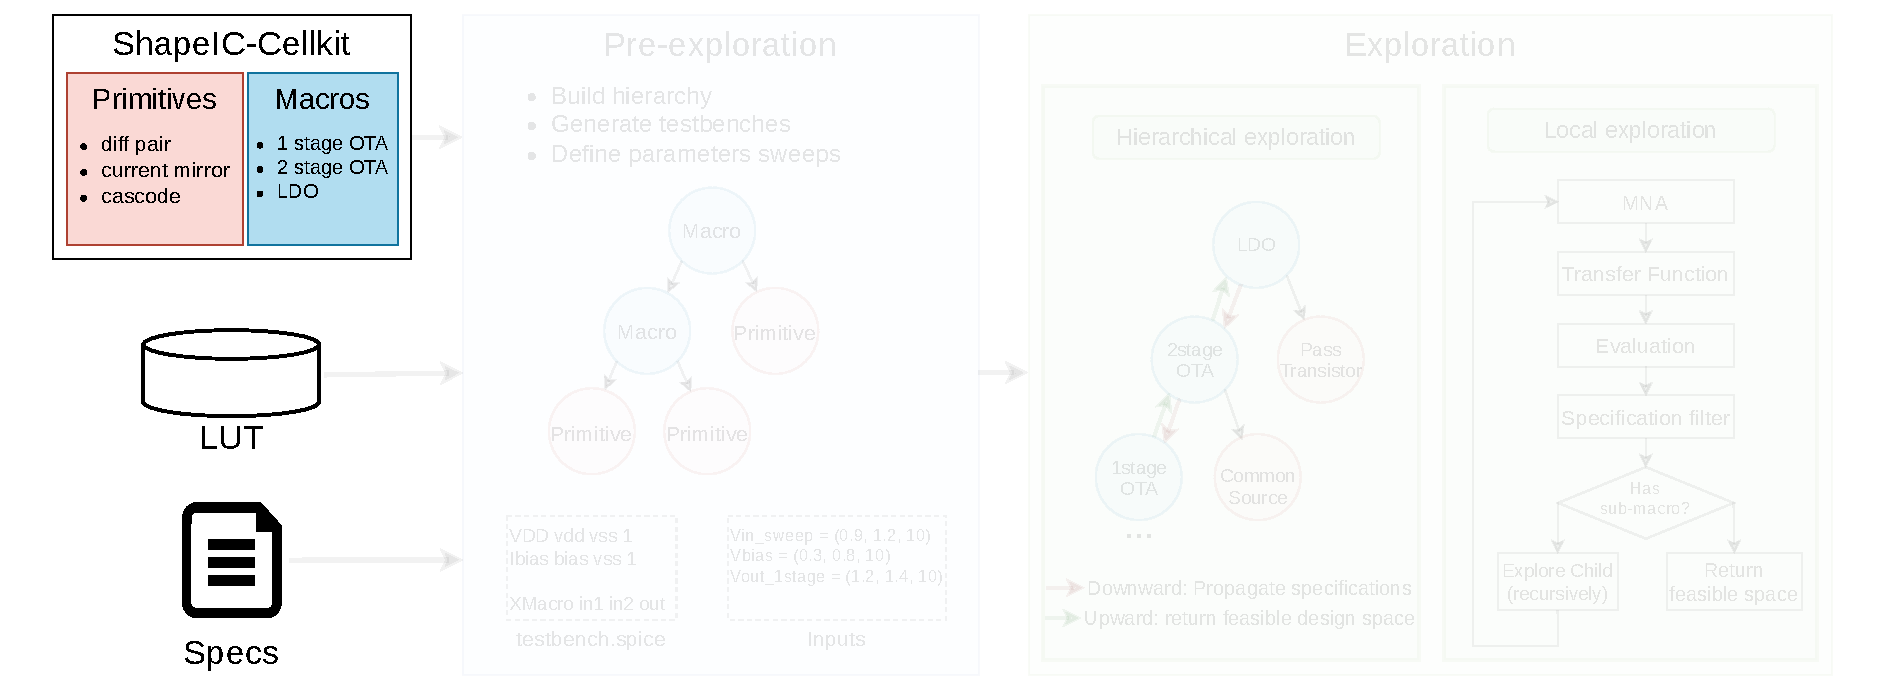
\includegraphics[width=1.15\textwidth]{img/shapeic-flow-p1.pdf}%
    }%
    \only<2>{%
      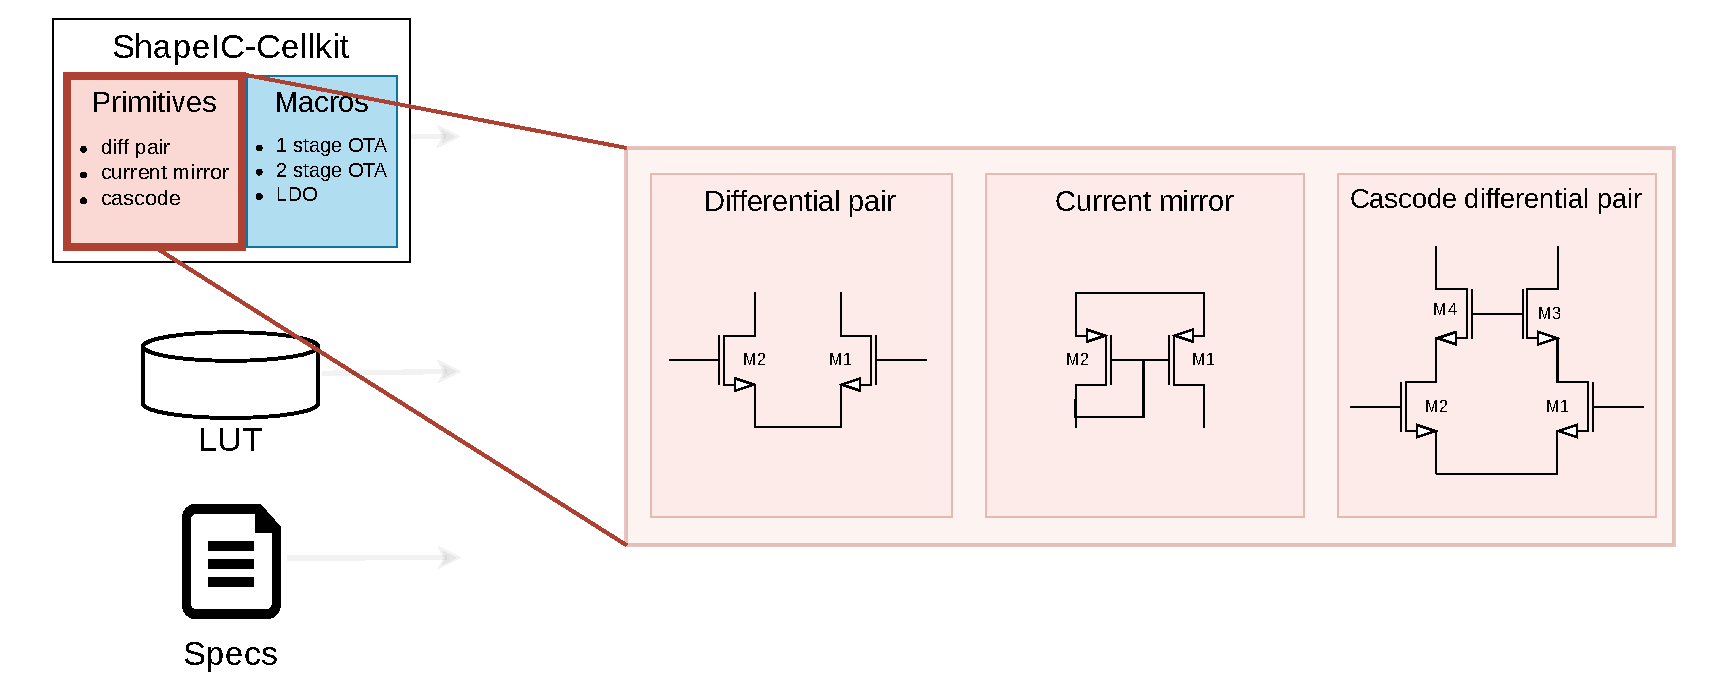
\includegraphics[width=1.15\textwidth]{img/shapeic-flow-p1.1.pdf}%
    }%
    \only<3>{%
      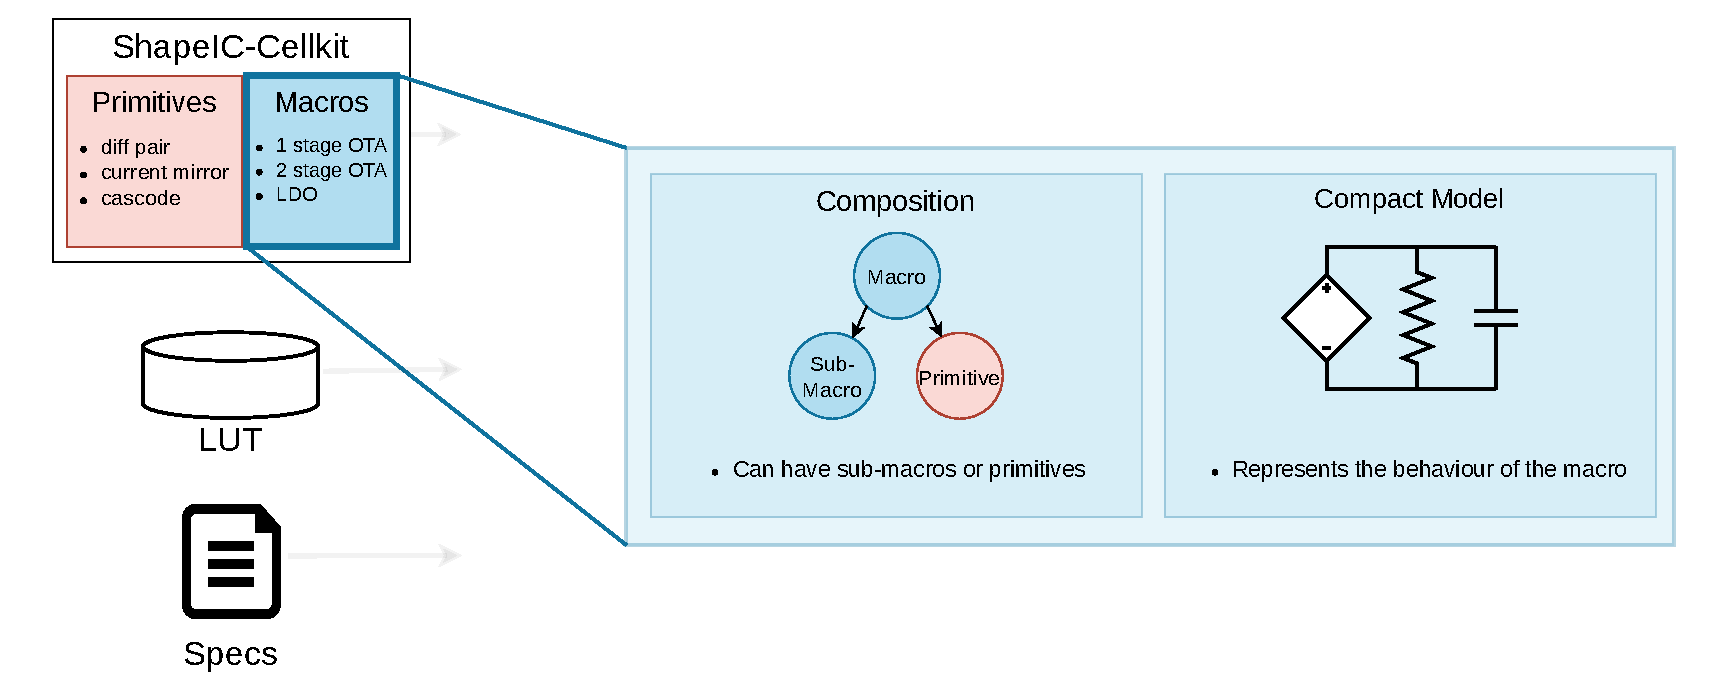
\includegraphics[width=1.15\textwidth]{img/shapeic-flow-p1.2.pdf}%
    }%
    \only<4>{%
      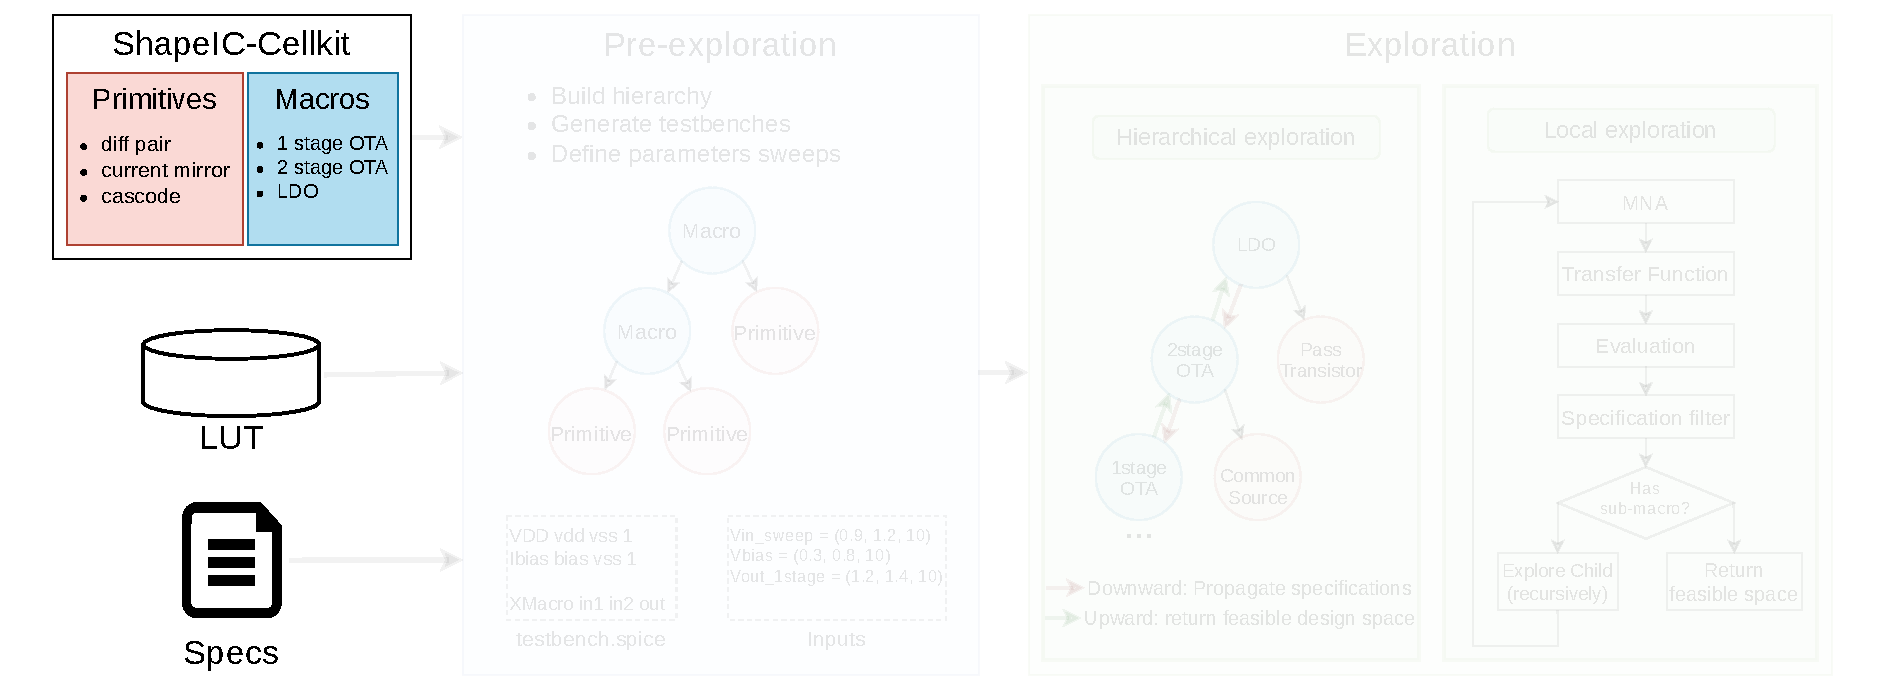
\includegraphics[width=1.15\textwidth]{img/shapeic-flow-p1.pdf}%
    }%
    \only<5>{%
      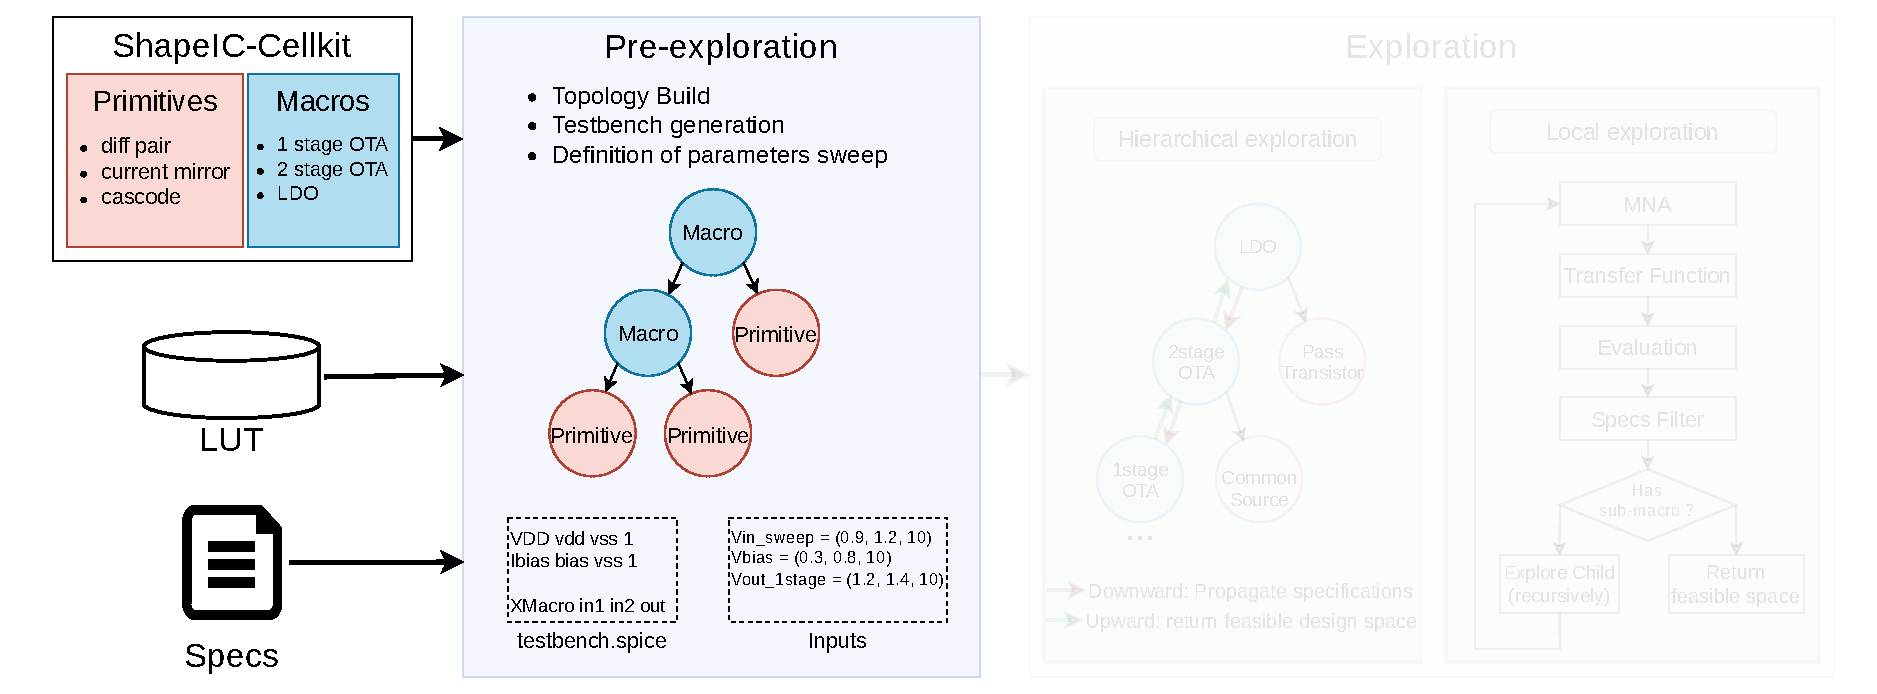
\includegraphics[width=1.15\textwidth]{img/shapeic-flow-p2.pdf}%
    }%
    \only<6>{%
      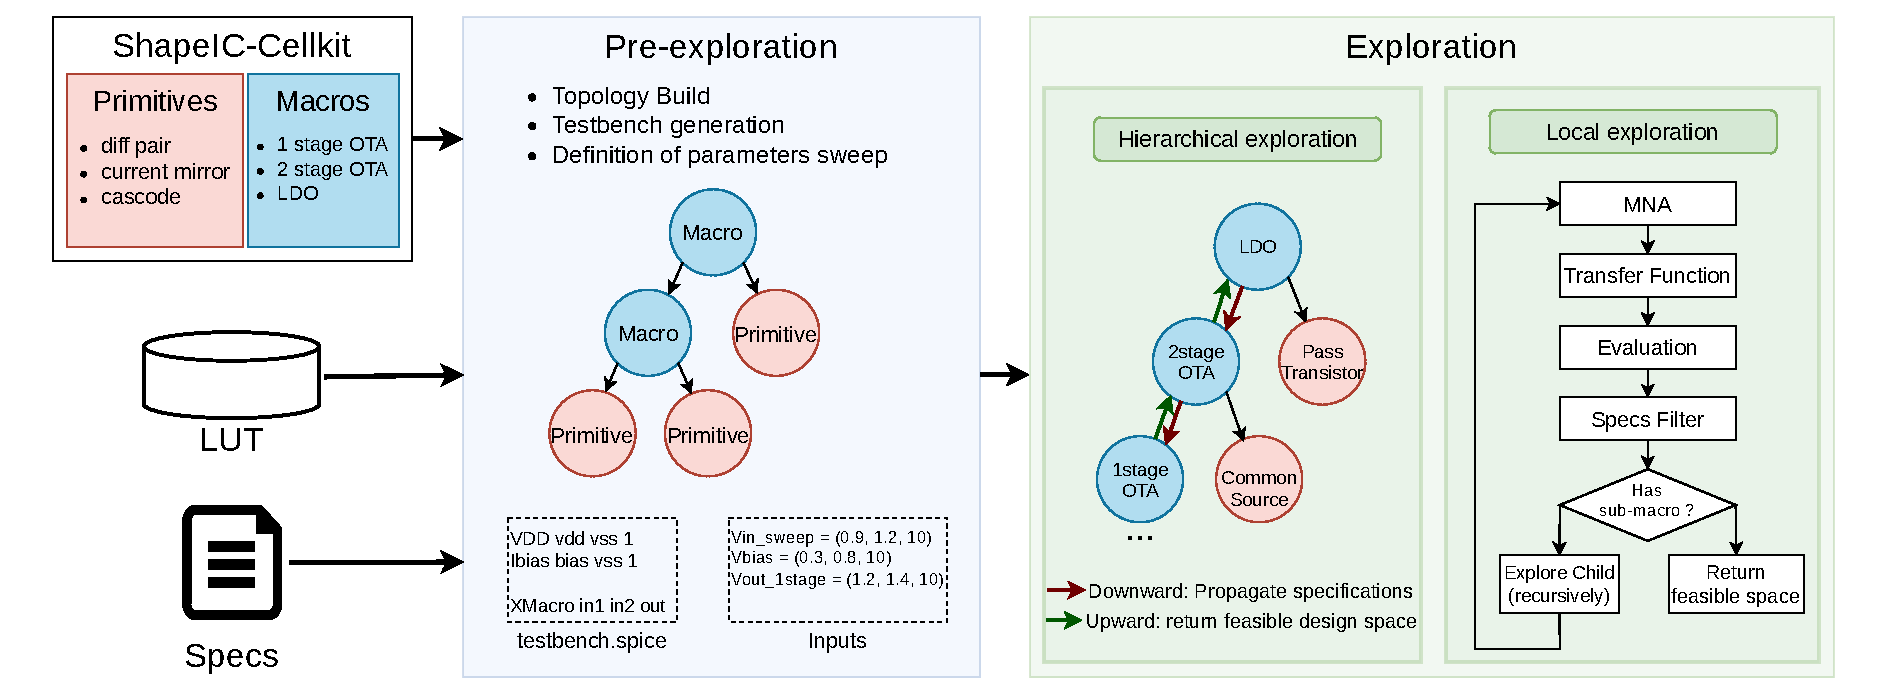
\includegraphics[width=1.15\textwidth]{img/shapeic-flow-p3.pdf}%
    }%
  }

\end{frame}

\section{ShapeIC in Action: 2 Stage Amplifier (OTA)}

\begin{frame}{ShapeIC in Action: 2 Stage Amplifier (OTA)}
\begin{columns}
    \begin{column}{0.45\textwidth}
      \center
      \only<5->{
        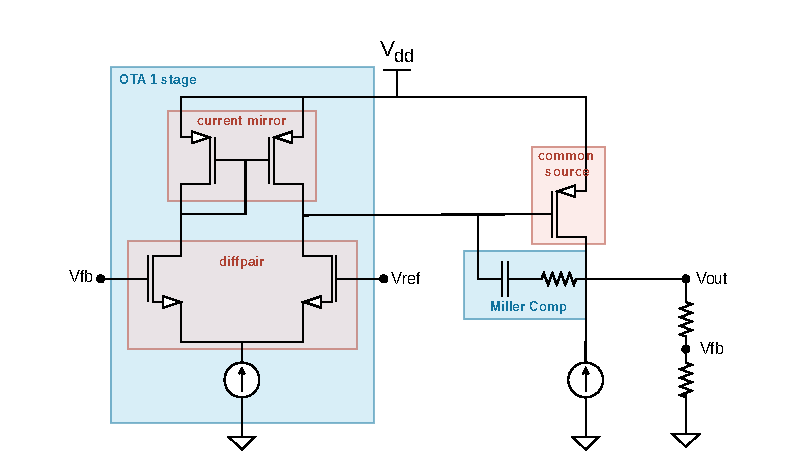
\includegraphics[width=\textwidth]{img/ota_2stage.pdf} 
        \begin{itemize}
          \item Testbench: AC analysis
          \item Specs: $Gain\geq70, BW\geq10kHz, PM\geq60$
        \end{itemize}
      }
      \only<1>{
        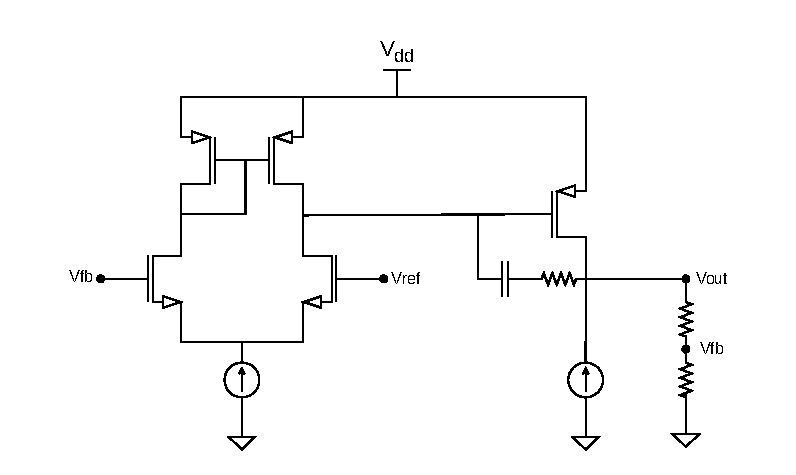
\includegraphics[width=\textwidth]{img/ota_2stage-pre.pdf} 
      }
      \only<2>{
        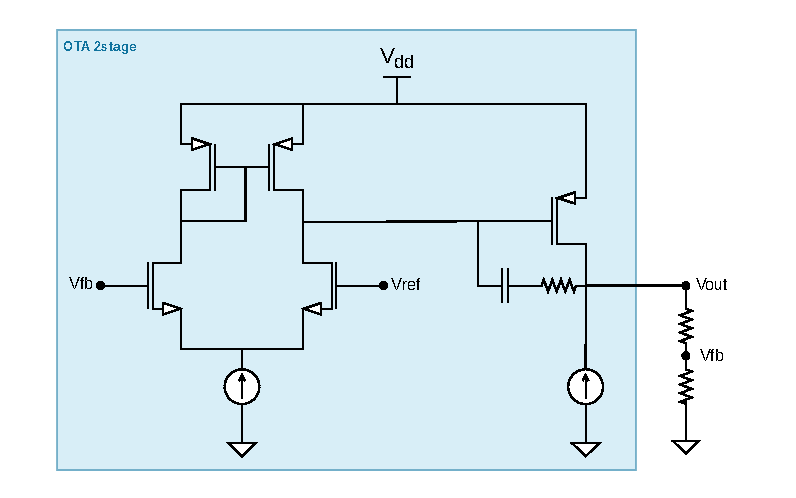
\includegraphics[width=\textwidth]{img/ota_2stage_p1.pdf} 
        \begin{itemize}
          \item Testbench: AC analysis
          \item Specs: $Gain\geq70, BW\geq10kHz, PM\geq60$
        \end{itemize}
      }
      \only<3>{
        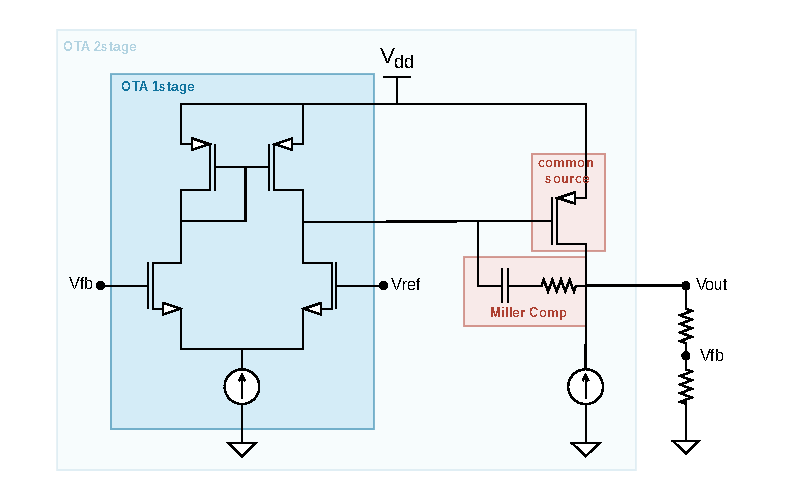
\includegraphics[width=\textwidth]{img/ota_2stage_p2.pdf} 
        \begin{itemize}
          \item Testbench: AC analysis
          \item Specs: $Gain\geq70, BW\geq10kHz, PM\geq60$
        \end{itemize}
      }
      \only<4>{
        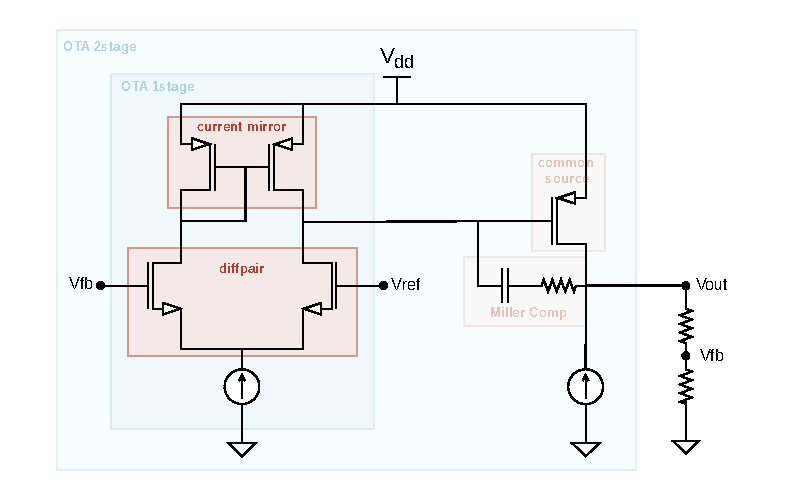
\includegraphics[width=\textwidth]{img/ota_2stage_p3.pdf} 
        \begin{itemize}
          \item Testbench: AC analysis
          \item Specs: $Gain\geq70, BW\geq10kHz, PM\geq60$
        \end{itemize}
      }
    \end{column}
    \begin{column}{0.45\textwidth}
      \only<4->{
          \center
          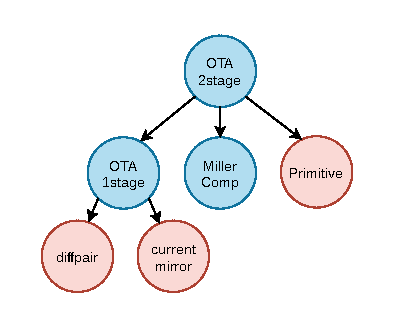
\includegraphics[width=\textwidth]{img/ota_2stage_hier.pdf} 
      }
      \only<2>{
          \center
          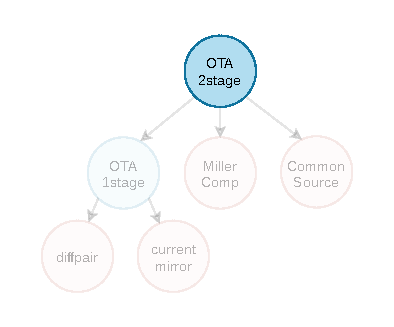
\includegraphics[width=\textwidth]{img/ota_2stage_hier_p1.pdf} 
      }
      \only<3>{
          \center
          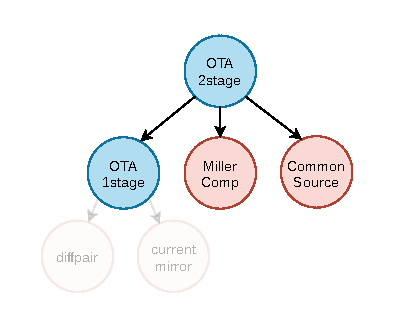
\includegraphics[width=\textwidth]{img/ota_2stage_hier_p2.pdf} 
      }
    \end{column}
\end{columns}
\only<2->{
  \begin{tikzpicture}[remember picture,overlay]
    \draw[->, ultra thick]
      ([xshift=-0.8cm,yshift=0.2cm]current page.center)
      --
      ([xshift=0.8cm,yshift=0.2cm]current page.center);
  \end{tikzpicture}
}
\end{frame}

\begin{frame}{ShapeIC in Action: 2 Stage Amplifier (OTA)}
\begin{columns}
  \begin{column}{0.45\textwidth}
      \begin{enumerate}
          \item<1-> Hierarchical exploration
            \begin{itemize}
              \item<1-> TOP exploration: $500k \rightarrow 2021$
                \begin{itemize}
                  \item<1-> Derived constraint: $Gain \geq 28.89\,[dB]$
                \end{itemize}
              \item<2-> Sub-macro exploration: $1050 \rightarrow 446$
                \begin{itemize}
                  \item<2-> Return to parent 446 candidates
                \end{itemize}
              \item<3-> TOP refresh: $223k \rightarrow 224$
            \end{itemize}
          \item<5-> Runtime
            \begin{itemize}
                \item Exploration only: $\approx 2.79s$
                \item Full run incl. LUT load: $\approx 8.38s$
          \end{itemize}

          \item<6-> {\color{red!70!black} Simulation-based optimization}
            \begin{itemize}
              \item<6-> {\color{red!70!black} Random initialization: no feasible solution found}
              \item<6-> {\color{red!70!black} ShapeIC-seeded initialization: converged to a feasible solution ($\star$)}
            \end{itemize}

      \end{enumerate}
  \end{column}

  \begin{column}{0.45\textwidth}
  \only<1>{
    \centering
    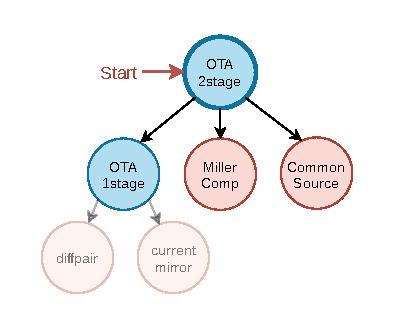
\includegraphics[width=\textwidth]{img/ota_2stage_exp_1.pdf} 
  }
  \only<2>{
    \centering
    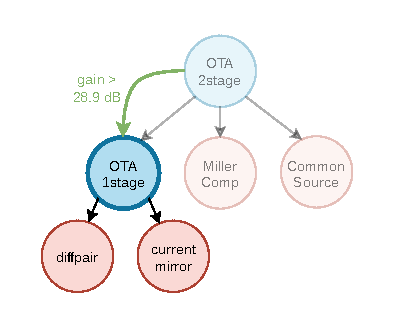
\includegraphics[width=\textwidth]{img/ota_2stage_exp_2.pdf} 
  }
  \only<3>{
    \centering
    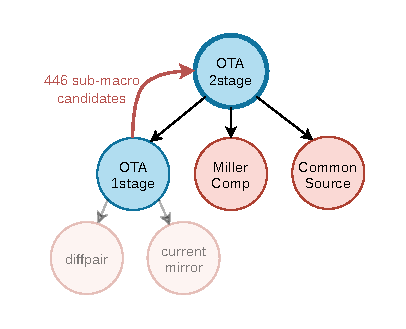
\includegraphics[width=\textwidth]{img/ota_2stage_exp_3.pdf} 
  }
  \only<4-5>{
    \centering
    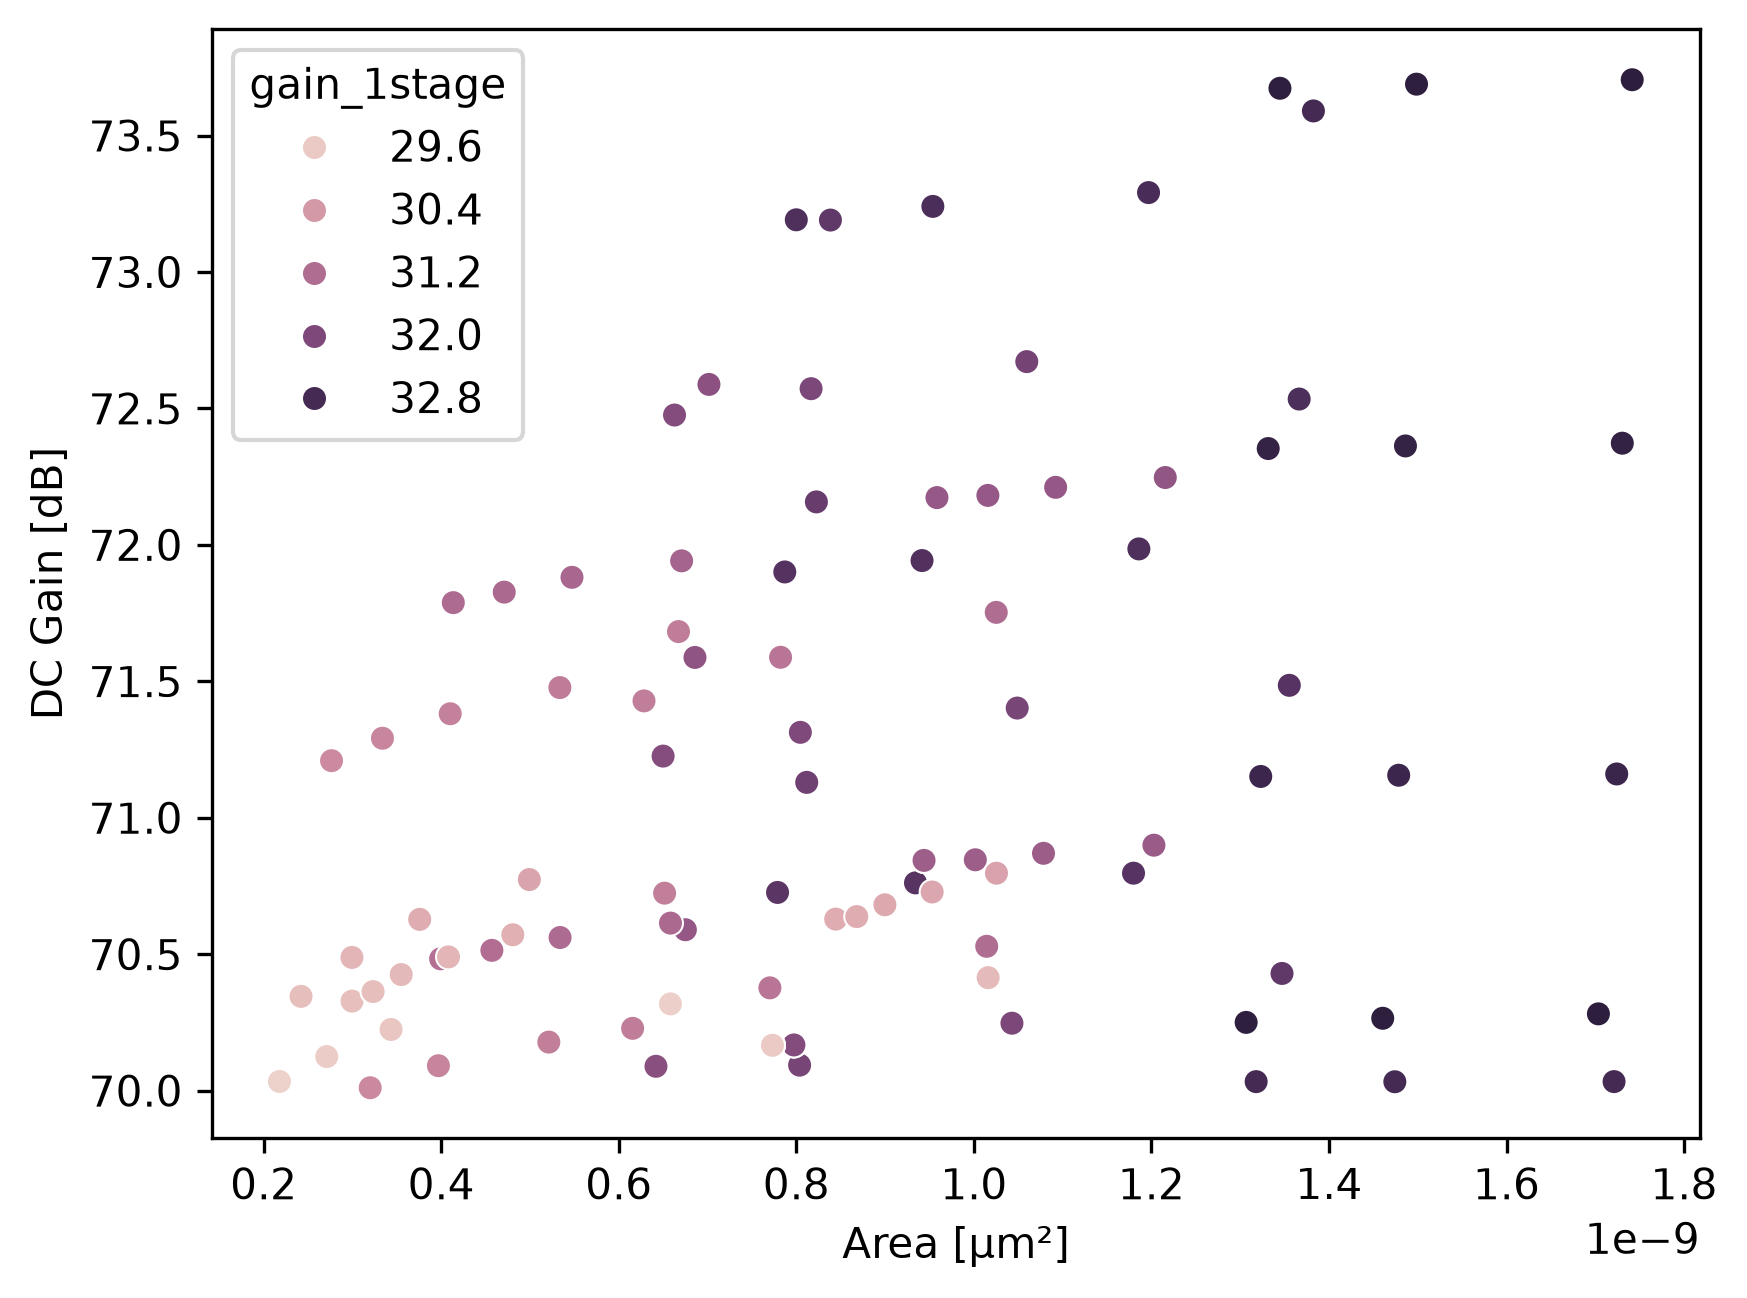
\includegraphics[width=\textwidth]{img/shapeic_exploration_onlygain.png} 
  }
  \only<6>{
    \centering
    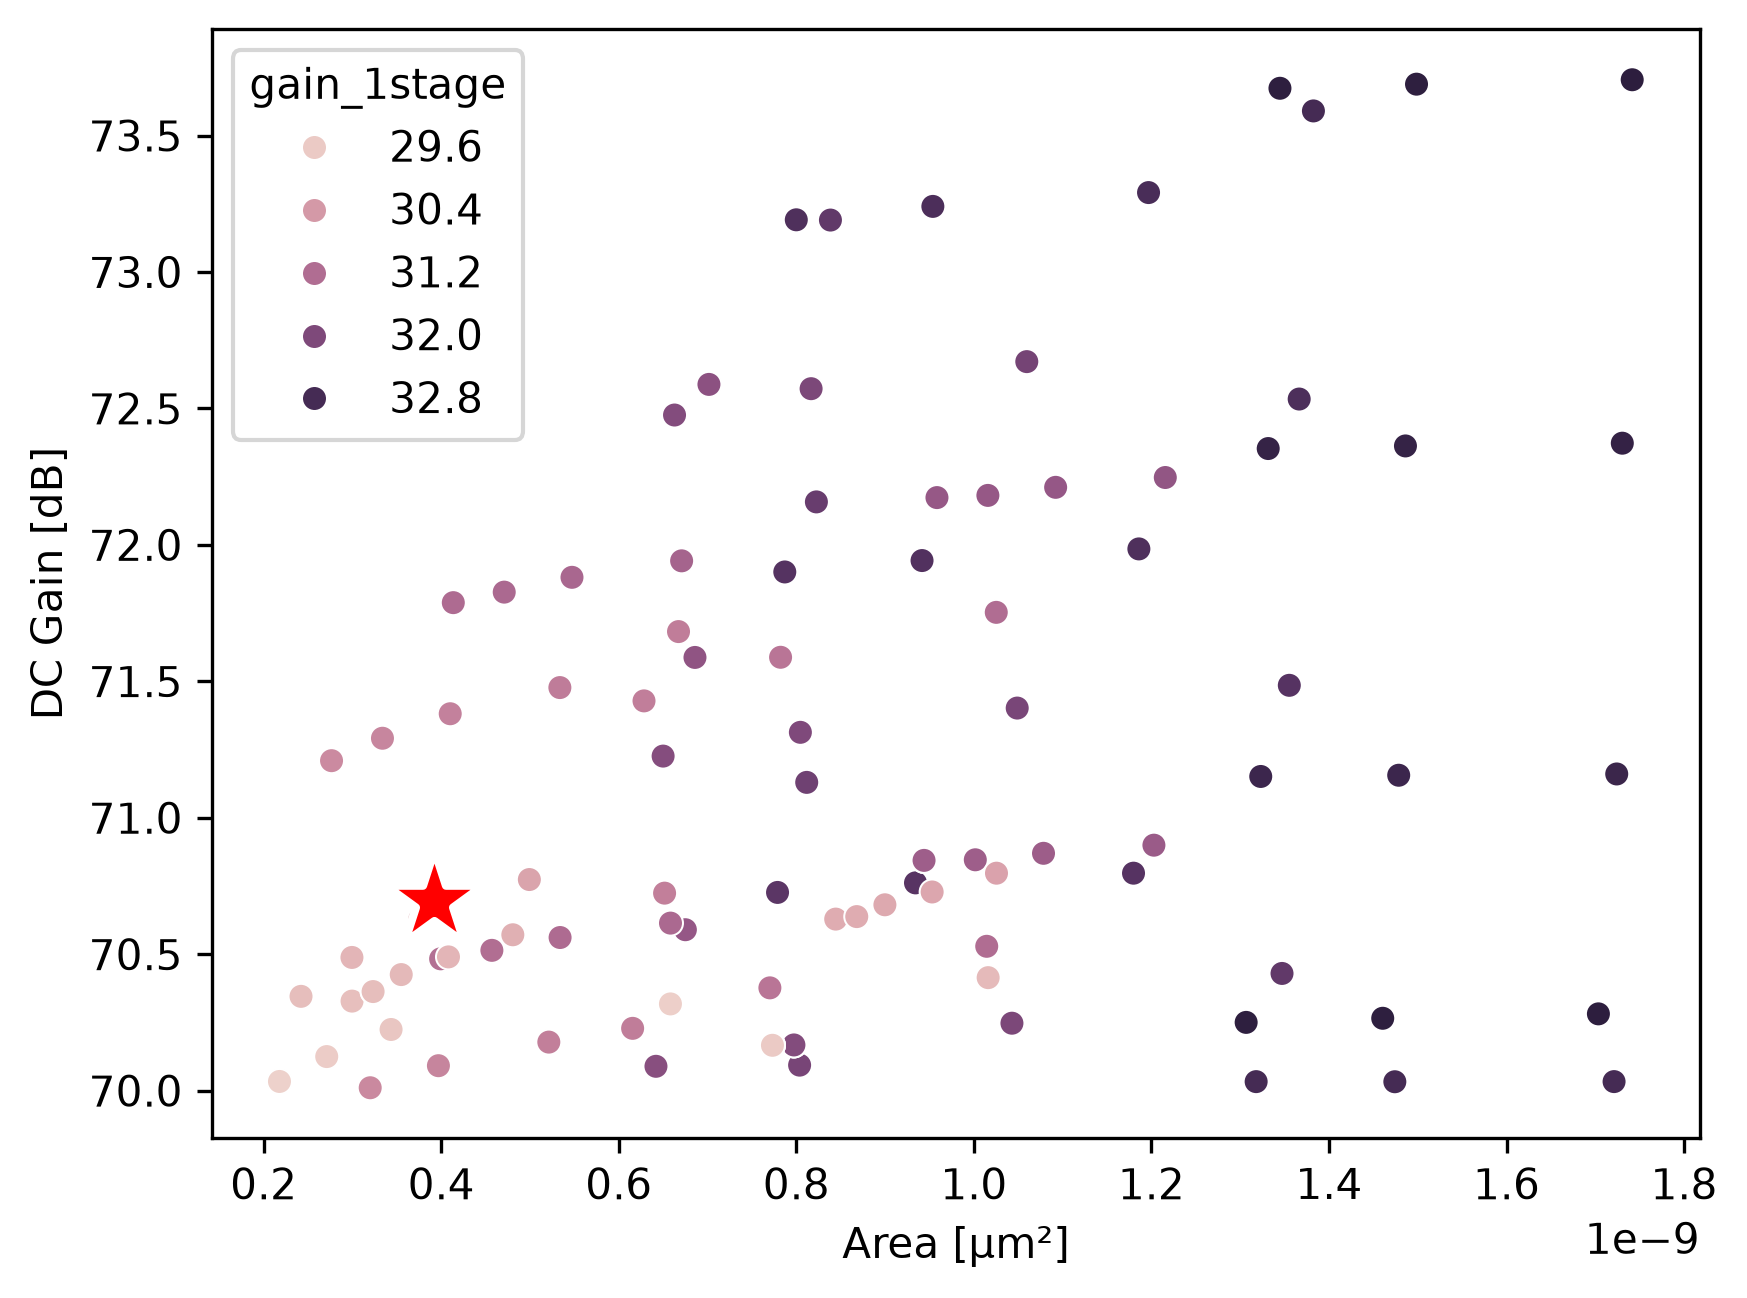
\includegraphics[width=\textwidth]{img/shapeic_exploration_onlygain_with_pyopus.png} 
  }
  \end{column}
\end{columns}
\end{frame}

\section{Current Status \& What is Next ?}

\begin{frame}{Current Status \& What is Next ?}
\begin{columns}
  \begin{column}{0.45\textwidth}
  \begin{itemize}
    \item Current status
      \begin{itemize}
        \item AC analysis supported 
        \item Hierarchycal LUT-based exploration
        \item Layout-aware exploration prototype
        \item ShapeIC-Cellkit integration
      \end{itemize}
  \end{itemize}
  \end{column}
  \begin{column}{0.45\textwidth}
  \begin{itemize}
    \item Current status
      \begin{itemize}
        \item AC analysis supported 
        \item Hierarchycal LUT-based exploration
        \item Layout-aware exploration prototype
        \item ShapeIC-Cellkit integration
      \end{itemize}
  \end{itemize}
  \end{column}
\end{columns}

\end{frame}

\end{document}
